\chapter{Methodology}\label{ch:methodology}
In this chapter, we are going to discuss the proposed framework and its main components in detail. The proposed method is efficient and computationally inexpensive compared to other methods proposed in literature. The workflow of the proposed network is illustrated in Figure~\ref{fig:overview_proposed_method}.

\begin{figure}
	\centering
	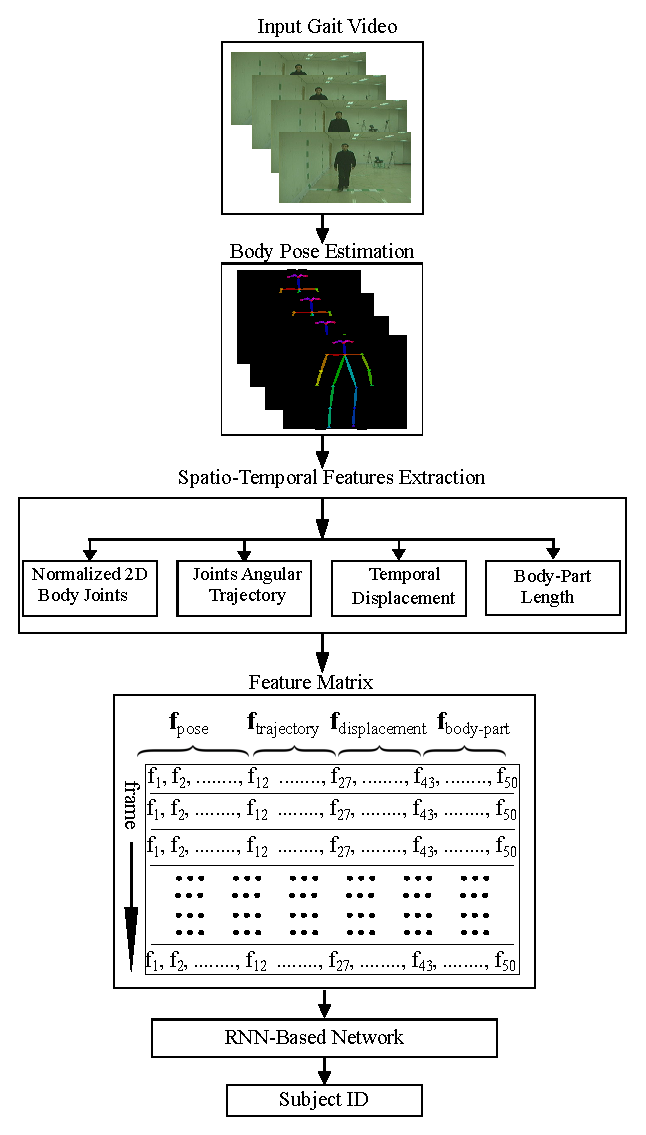
\includegraphics[width=0.8\textwidth]{figures/proposed_method.eps}
	\caption [The overview of the proposed framework for gait recognition] 
	{The overview of the proposed framework for gait recognition. 2D human poses were first extracted from raw video frames using improved OpenPose~\cite{Cao_19} algorithm. Four different types of spatio-temporal features were then extracted to form a 50-dimensional feature vector. Thereafter a pose sequence of timestep each having a length of 28 frame was formed to feed into a temporal network. The temporal network identified the subject by modeling the gait features. \label{fig:overview_proposed_method}
	}	
\end{figure}


%-------------------------------------------------------------------------
\section{Deep Learning Basics}
\subsection{Recurrent Neural Network} 
The Recurrent Neural Network (\gls{rnn}) is neural sequence model that achieves state of the art performance on important tasks that include language modeling~\cite{mikolov_12}, speech recognition~\cite{graves_13}, and machine translation~\cite{kal_13}.  

It is well known that the brain is organized in functional areas and sub-areas that process the incoming signal in an incremental fashion. These areas of the brain are typically connected both in a \emph{feedforward}, i.e., towards
neurons belonging to deeper (i.e., further away from the sensory input) layers, and in a \emph{feedback} fashion (i.e., to previous layers in the hierarchy). This is believed to help processing temporal data and allow for an iterative refinement of the computation.

Similarly, ANNs are not constrained to process the input data in a feedforward way. Recurrent Neural Networks (\gls{rnn}s) implement feedback loops (see~\ref{fig:RNN_loop} \footnote{This and the following RNN figures, are taken or modified from the awesome introduction to RNNs and LSTMs by Chris Olah~\cite{colah_15}}) that propagate some information from one step to the next. It is customary to refer to these steps as time-steps, as RNNs are often considered in the context of a discretized time evolving domain, but nothing prevents from using RNNs with any kind of sequential data.

\begin{figure}[t]
	\centering
	\includegraphics[width=0.15\textwidth]{figures/RNN_loop.pdf}
	\caption{A Recurrent Neural Network (RNN).\label{fig:RNN_loop}}
\end{figure}

\begin{figure}[t!]
	\centering
	\includegraphics[width=0.7\textwidth]{figures/RNN_unrolled.pdf}
	\caption{A Recurrent Neural Network unrolled for $t$\% steps.\label{fig:RNN_unrolled}}
\end{figure}

Suppose to model some sequential data $x_0, x_1, \dots , x_t, x_{t+1}, \dots$ such as an English sentence. At time $t$ it is possible to model the probability distribution over a dictionary of English words, conditioned on the words seen up that moment -- namely $x_0, x_1, \dots , x_{t-1}$. This can be used, for instance, in a smart keyboard application to suggest the next most probable words to the user or, in an automatic help desk, to generate a meaningful answer to a question.

It might not be immediately obvious what it means in practice to put a loop in an ANN and how to backpropagate through it. To better comprehend how RNNs work it is useful to consider its behavior explicitly by \emph{unrolling} the RNN, as shown in~\ref{fig:RNN_unrolled}

An RNN applies the same model to each time step of the sequence or, equivalently, applies different models at each time step, which share their weights. This is similar to what CNNs do over space with convolutions, but is rather done over time with feedback connections.

The activation of an RNN (see~\ref{fig:RNN_unrolled}) at time $t$ depends on the input at time $t$ as well as on the information coming from the previous step $t-1$. RNNs have a very simple internal structure, that usually amounts to applying some affine transformation to the input and to the previous output, and computing some non-linearity (typically a $tanh$) of their sum.

One of the key benefits of RNNs is their ability to make use of previous context.   However,  for standard RNN architectures, the range of context that can in practice be accessed is limited.  The problem is that the influence of a given input on the hidden layer,  and therefore on the network output, either decays or blows up exponentially as it cycles around the recurrent connections.  This is often referred to as the \textit{vanishing gradient problem}~\cite{Hochreiter_01}. 

\begin{figure}[t]
	\centering
	\includegraphics[width=0.7\textwidth]{figures/RNN_internals.pdf}
	\includegraphics[width=0.7\textwidth]{figures/LSTM_notation.pdf}
	\caption{The internal structure of an RNN.\label{fig:RNN_internals}}
\end{figure}

To train it it suffices to unroll the computation graph and use the backpropagation algorithm to proceed from the most recent time step, backward in time. This algorithm is usually referred to as \emph{Backpropagation through time (BPTT)}.

The problem of BPTT is that it requires the application of the chain rule all the way from the current time step to $t = 0$ to propagate the gradients through time.  This results in a long chain of products that can easily go to
infinity or become zero if the elements of the multiplication are greater or smaller than $1$ respectively. These two issues, i.e., going to infinity and becoming zero, are known in the literature as \emph{exploding gradient} and \emph{vanishing gradient} respectively, and have been studied extensively in the past, see e.g.,~\cite{Bengio_94}. The first one can be partially addressed by \emph{clipping the gradient} when it becomes too large, but the second is not easy to overcome and can make training these kind of models very hard if not impossible.

\subsection{Long Short Term Memory}\label{sec:LSTM}
\begin{figure}[t]
	\centering
	\includegraphics[width=0.7\textwidth]{figures/LSTM.pdf}
	\caption{A Long Short Term Memory (LSTM).\label{fig:LSTM}}
\end{figure}

Long Short Term Memory (LSTM) networks (see~\ref{fig:LSTM}) have been proposed to solve (or at least alleviate) the problems of RNNs in modeling long term dependencies. LSTMs have been designed to have an internal memory, or~\emph{state}, that can be updated and consulted at each time step. As opposed to vanilla RNNs, this allows LSTMs to separate their output from the information they want to carry over to future steps.

\begin{figure}[t]
	\centering
	\includegraphics[width=0.6\textwidth]{figures/LSTM_state.pdf}
	\caption{The internal state of LSTMs.\label{fig:LSTM_state}}
\end{figure}

\ref{fig:LSTM_state} highlights the internal memory path. It can be seen how the internal memory of the previous time step $\mathbf{c}_{t-1}$ is carried over to the current time step, where it is updated through a multiplicative and an additive interaction and concurs to determine the current state of the memory $\mathbf{c}_t$. This is then, once again, propagated to the next time step.


\begin{figure}[p]
	\centering
	\includegraphics[width=0.5\textwidth]{figures/LSTM_forget_gate.pdf}
	\caption{The LSTM forget gate.\label{fig:LSTM_forget_gate}}
\end{figure}
\begin{figure}[p]
	\centering
	\includegraphics[width=0.5\textwidth]{figures/LSTM_input_gate.pdf}
	\caption{The LSTM input gate.\label{fig:LSTM_input_gate}}
\end{figure}
\begin{figure}[p]
	\centering
	\includegraphics[width=0.5\textwidth]{figures/LSTM_output_gate.pdf}
	\caption{The LSTM output gate.\label{fig:LSTM_output_gate}}
\end{figure}

LSTMs interact with memory through \emph{gates}, computational nodes that determine the behavior of the model. The \emph{forget~gate}~(\ref{fig:LSTM_forget_gate}) determines how much of the previous step's memory to forget or, equivalently, how much of the previous state to retain.  This is modeled through a sigmoid layer (depicted as $\sigma$) that takes the current input $\mathbf{x}_t$ and the output of the previous step $\mathbf{h}_{t-1}$ and produces an activation vector between $0$ and $1$

\begin{equation}\label{eq:LSTM_forget_gate}
\mathbf{f}_t = \sigma\left(\mathbf{W}_f \cdot \mathbf{h}_{t-1} +
\mathbf{W}_f \cdot \mathbf{x}_t + \mathbf{b}_f \right),
\end{equation}

this activation is multiplied by the previous state $\mathbf{c}_{t-1}$ and results in an intermediate memory state where some of the activations can be weaker than those in $\mathbf{c}_{t-1}$ and some others are potentially zeroed out.

The forget gate allows the LSTM to discard information that is not relevant anymore. Symmetrically, LSTMs have a mechanism to add new information to the memory. This behavior is controlled by an \emph{input gate} (see
\ref{fig:LSTM_input_gate}) that modulates the amount of the current input that is going to be stored in the memory. This operation is split over two computation paths: similarly to the forget gate, the input gate takes the current input $\mathbf{x}_t$ and the output of the previous step $\mathbf{h}_{t-1}$ and exploits a sigmoid layer to produce an activation vector between $0$ and $1$.  Simultaneously, a $tanh$ layer generates a state update $\mathbf{\tilde c}_t$ between $-1$ and $1$. This is governed by the equations

\begin{equation}\label{eq:LSTM_input_gate}
\begin{split}
\mathbf{i}_t &= \sigma\left(\mathbf{W}_i \cdot \mathbf{h}_{t-1} +
\mathbf{W}_i \cdot \mathbf{x}_t + \mathbf{b}_i \right),\\
\mathbf{\tilde c}_t &= tanh \left(\mathbf{W}_c \cdot
\mathbf{h}_{t-1} + \mathbf{W}_c \cdot \mathbf{x}_t +
\mathbf{b}_c \right).
\end{split}
\end{equation}

The input gate modulates how much of this state update will be applied to the old state to generate the current state. The forget gate $\mathbf{f}_t$ and the input gate $\mathbf{i}_t$, together with the state update $\mathbf{\tilde c}_t$ and the previous state $\mathbf{c}_{t-1}$ fully determine the state at time $t$ through

\begin{equation}\label{eq:LSTM_state_update}
\mathbf{c}_t = \mathbf{f}_t \circ \mathbf{c}_{t-1} +
\mathbf{i}_t \circ \mathbf{\tilde c}_t.
\end{equation}

The last gate of LSTMs is the \emph{output~gate}~(\ref{fig:LSTM_output_gate}) $\mathbf{o}_t$ that, as the name reveals, manipulates the output of the LSTM at time $t$. The usual sigmoid layer determines the state of the output gate

\begin{equation}\label{eq:LSTM_output_gate}
\begin{split}
\mathbf{o}_t &= \sigma\left(\mathbf{W}_o \cdot \mathbf{h}_{t-1} +
\mathbf{W}_o \cdot \mathbf{x}_t + \mathbf{b}_o \right),\\
\mathbf{h}_t &= \mathbf{o}_t \circ tanh \left(\mathbf{c}_t\right),
\end{split}
\end{equation}

and the memory resulting from the transformations due to the forget and input gates goes through a $tanh$ nonlinearity and is multiplied by the output gate to finally produce the output.

Putting it all together, the equations that govern the behavior of an LSTM are

\begin{equation}\label{eq:LSTM}
\begin{split}
\mathbf{i}_t &= \sigma\left(\mathbf{W}_i \cdot \mathbf{h}_{t-1} +
\mathbf{W}_i \cdot \mathbf{x}_t + \mathbf{b}_i \right),\\
\mathbf{f}_t &= \sigma\left(\mathbf{W}_f \cdot \mathbf{h}_{t-1} +
\mathbf{W}_f \cdot \mathbf{x}_t + \mathbf{b}_f \right),\\
\mathbf{\tilde c}_t &= tanh \left(\mathbf{W}_c \cdot \mathbf{h}_{t-1} +
\mathbf{W}_c \cdot \mathbf{x}_t + \mathbf{b}_c \right),\\
\mathbf{c}_t &= \mathbf{f}_t \circ \mathbf{c}_{t-1} + \mathbf{i}_t
\circ \mathbf{\tilde c}_t,\\
\mathbf{o}_t &= \sigma\left(\mathbf{W}_o \cdot \mathbf{h}_{t-1} +
\mathbf{W}_o \cdot \mathbf{x}_t + \mathbf{b}_o \right),\\
\mathbf{h}_t &= \mathbf{o}_t \circ tanh \left(\mathbf{c}_t\right).
\end{split}
\end{equation}


\subsubsection{LSTMs with peepholes}

\cite{gers_00} suggests one variant of LSTMs where the gates also have information about the state of the LSTM. Note that, as illustrated in~\ref{fig:LSTM_peepholes}, the output gate peeps into $\mathbf{c}_t$, i.e., the state after the input and forget gate updates

\begin{figure}
	\centering
	\includegraphics[width=0.6\textwidth]{figures/LSTM_peepholes.pdf}
	\caption{LSTM with peepholes.\label{fig:LSTM_peepholes}}
\end{figure}

\begin{equation}\label{eq:LSTM_peepholes}
\begin{split}
\mathbf{i}_t &= \sigma\left(\mathbf{W}_i \cdot \mathbf{h}_{t-1} +
\mathbf{W}_i \cdot \mathbf{x}_t +
\mathbf{W}_{ic} \circ \mathbf{c}_{t-1} +
\mathbf{b}_i \right),\\
\mathbf{f}_t &= \sigma\left(\mathbf{W}_f \cdot \mathbf{h}_{t-1} +
\mathbf{W}_f \cdot \mathbf{x}_t +
\mathbf{W}_{fc} \circ \mathbf{c}_{t-1} +
\mathbf{b}_f \right),\\
\mathbf{\tilde c}_t &= tanh \left(\mathbf{W}_c \cdot \mathbf{h}_{t-1} +
\mathbf{W}_c \cdot \mathbf{x}_t + \mathbf{b}_c \right),\\
\mathbf{c}_t &= \mathbf{f}_t \circ \mathbf{c}_{t-1} + \mathbf{i}_t
\circ \mathbf{\tilde c}_t,\\
\mathbf{o}_t &= \sigma\left(\mathbf{W}_o \cdot \mathbf{h}_{t-1} +
\mathbf{W}_o \cdot \mathbf{x}_t +
\mathbf{W}_{oc} \circ \mathbf{c}_{t} +
\mathbf{b}_o \right),\\
\mathbf{h}_t &= \mathbf{o}_t \circ tanh \left(\mathbf{c}_t\right).
\end{split}
\end{equation}


\subsubsection{LSTMs with coupled forget and input gates}\label{sec:LSTM_coupled}

Another variant of LSTMs~\cite{Greff_15} replaces the input gate with $1 - \mathbf{f}_t$ (see~\ref{fig:LSTM_coupled}), so that the forget gate governs both behaviors. This boils down to forgetting only when a new input is going to be written. The modified state update equation is

\begin{equation}\label{eq:LSTM_coupled}
\mathbf{c}_t = \mathbf{f}_t \circ \mathbf{c}_{t-1} + (1 - \mathbf{f}_t)
\circ \mathbf{\tilde c}_t.
\end{equation}

\begin{figure}
	\centering
	\includegraphics[width=0.6\textwidth]{figures/LSTM_coupled.pdf}
	\caption{LSTM with coupled forget and input gate.\label{fig:LSTM_coupled}}
\end{figure}


\subsection{Gated Recurrent Unit (GRU)}\label{sec:GRU}

In 2014 \cite{Cho_14} proposed a new kind of recurrent network called Gated Recurrent Unit (GRU) (see~\ref{fig:GRU}) with less gates than LSTMs and a different internal structure. Along the lines of \ref{sec:LSTM_coupled}, in GRUs the forget and input gates are coupled into an~\emph{update gate} $\mathbf{z}_t$.  The memory and output are also merged into a single state and the internal structure is modified to cope with these changes

\begin{figure}
	\centering
	\includegraphics[width=0.6\textwidth]{figures/GRU.pdf}
	\caption{Gated Recurrent Units (GRUs).\label{fig:GRU}}
\end{figure}

\begin{equation}\label{eq:GRU}
\begin{split}
\mathbf{z}_t &= \sigma \left(\mathbf{W}_z \cdot \mathbf{h}_{t-1} +
\mathbf{W}_z \cdot \mathbf{x}_t\right), \\
\mathbf{r}_t &= \sigma \left(\mathbf{W}_r \cdot \mathbf{h}_{t-1} +
\mathbf{W}_r \cdot \mathbf{x}_t\right), \\
\mathbf{\tilde h}_t &= tanh \left(
\mathbf{W}_o \cdot \mathbf{r}_t + \circ \mathbf{h}_{t-1} +
\mathbf{W}_o \cdot \mathbf{x}_t
\right), \\
\mathbf{h}_t &= (1-\mathbf{z}_t) \circ \mathbf{h}_{t-1} +
(\mathbf{z}_t) \circ \mathbf{\tilde h}_t.
\end{split}
\end{equation}

The advantage of GRUs over LSTMs is the smaller number of gates that makes them less memory as well as computationally intense, which is often a critical aspect for ANNs. GRUs have been shown to perform as well as LSTMs in some settings.

\subsection{Bidirectional RNNs}
Bidirectional recurrent neural networks (\gls{brnn}) connect two hidden layers running in opposite directions to a single output, allowing them to receive information from both past and future states. Here, the input sequence is fed in normal time order for one network, and in reverse time order for another. The outputs of the two networks are usually concatenated at each time step. So, this type of structure allows the networks to have both backward and forward information about the sequence at every time step. \gls{brnn} are especially useful when the context of the input is needed. For example, in handwriting recognition~\cite{Graves_08}, the performance can be enhanced by knowledge of the letters located before and after the current letter. 




\subsubsection{Bidirectional Vanilla RNN}
\begin{figure}
	\centering
	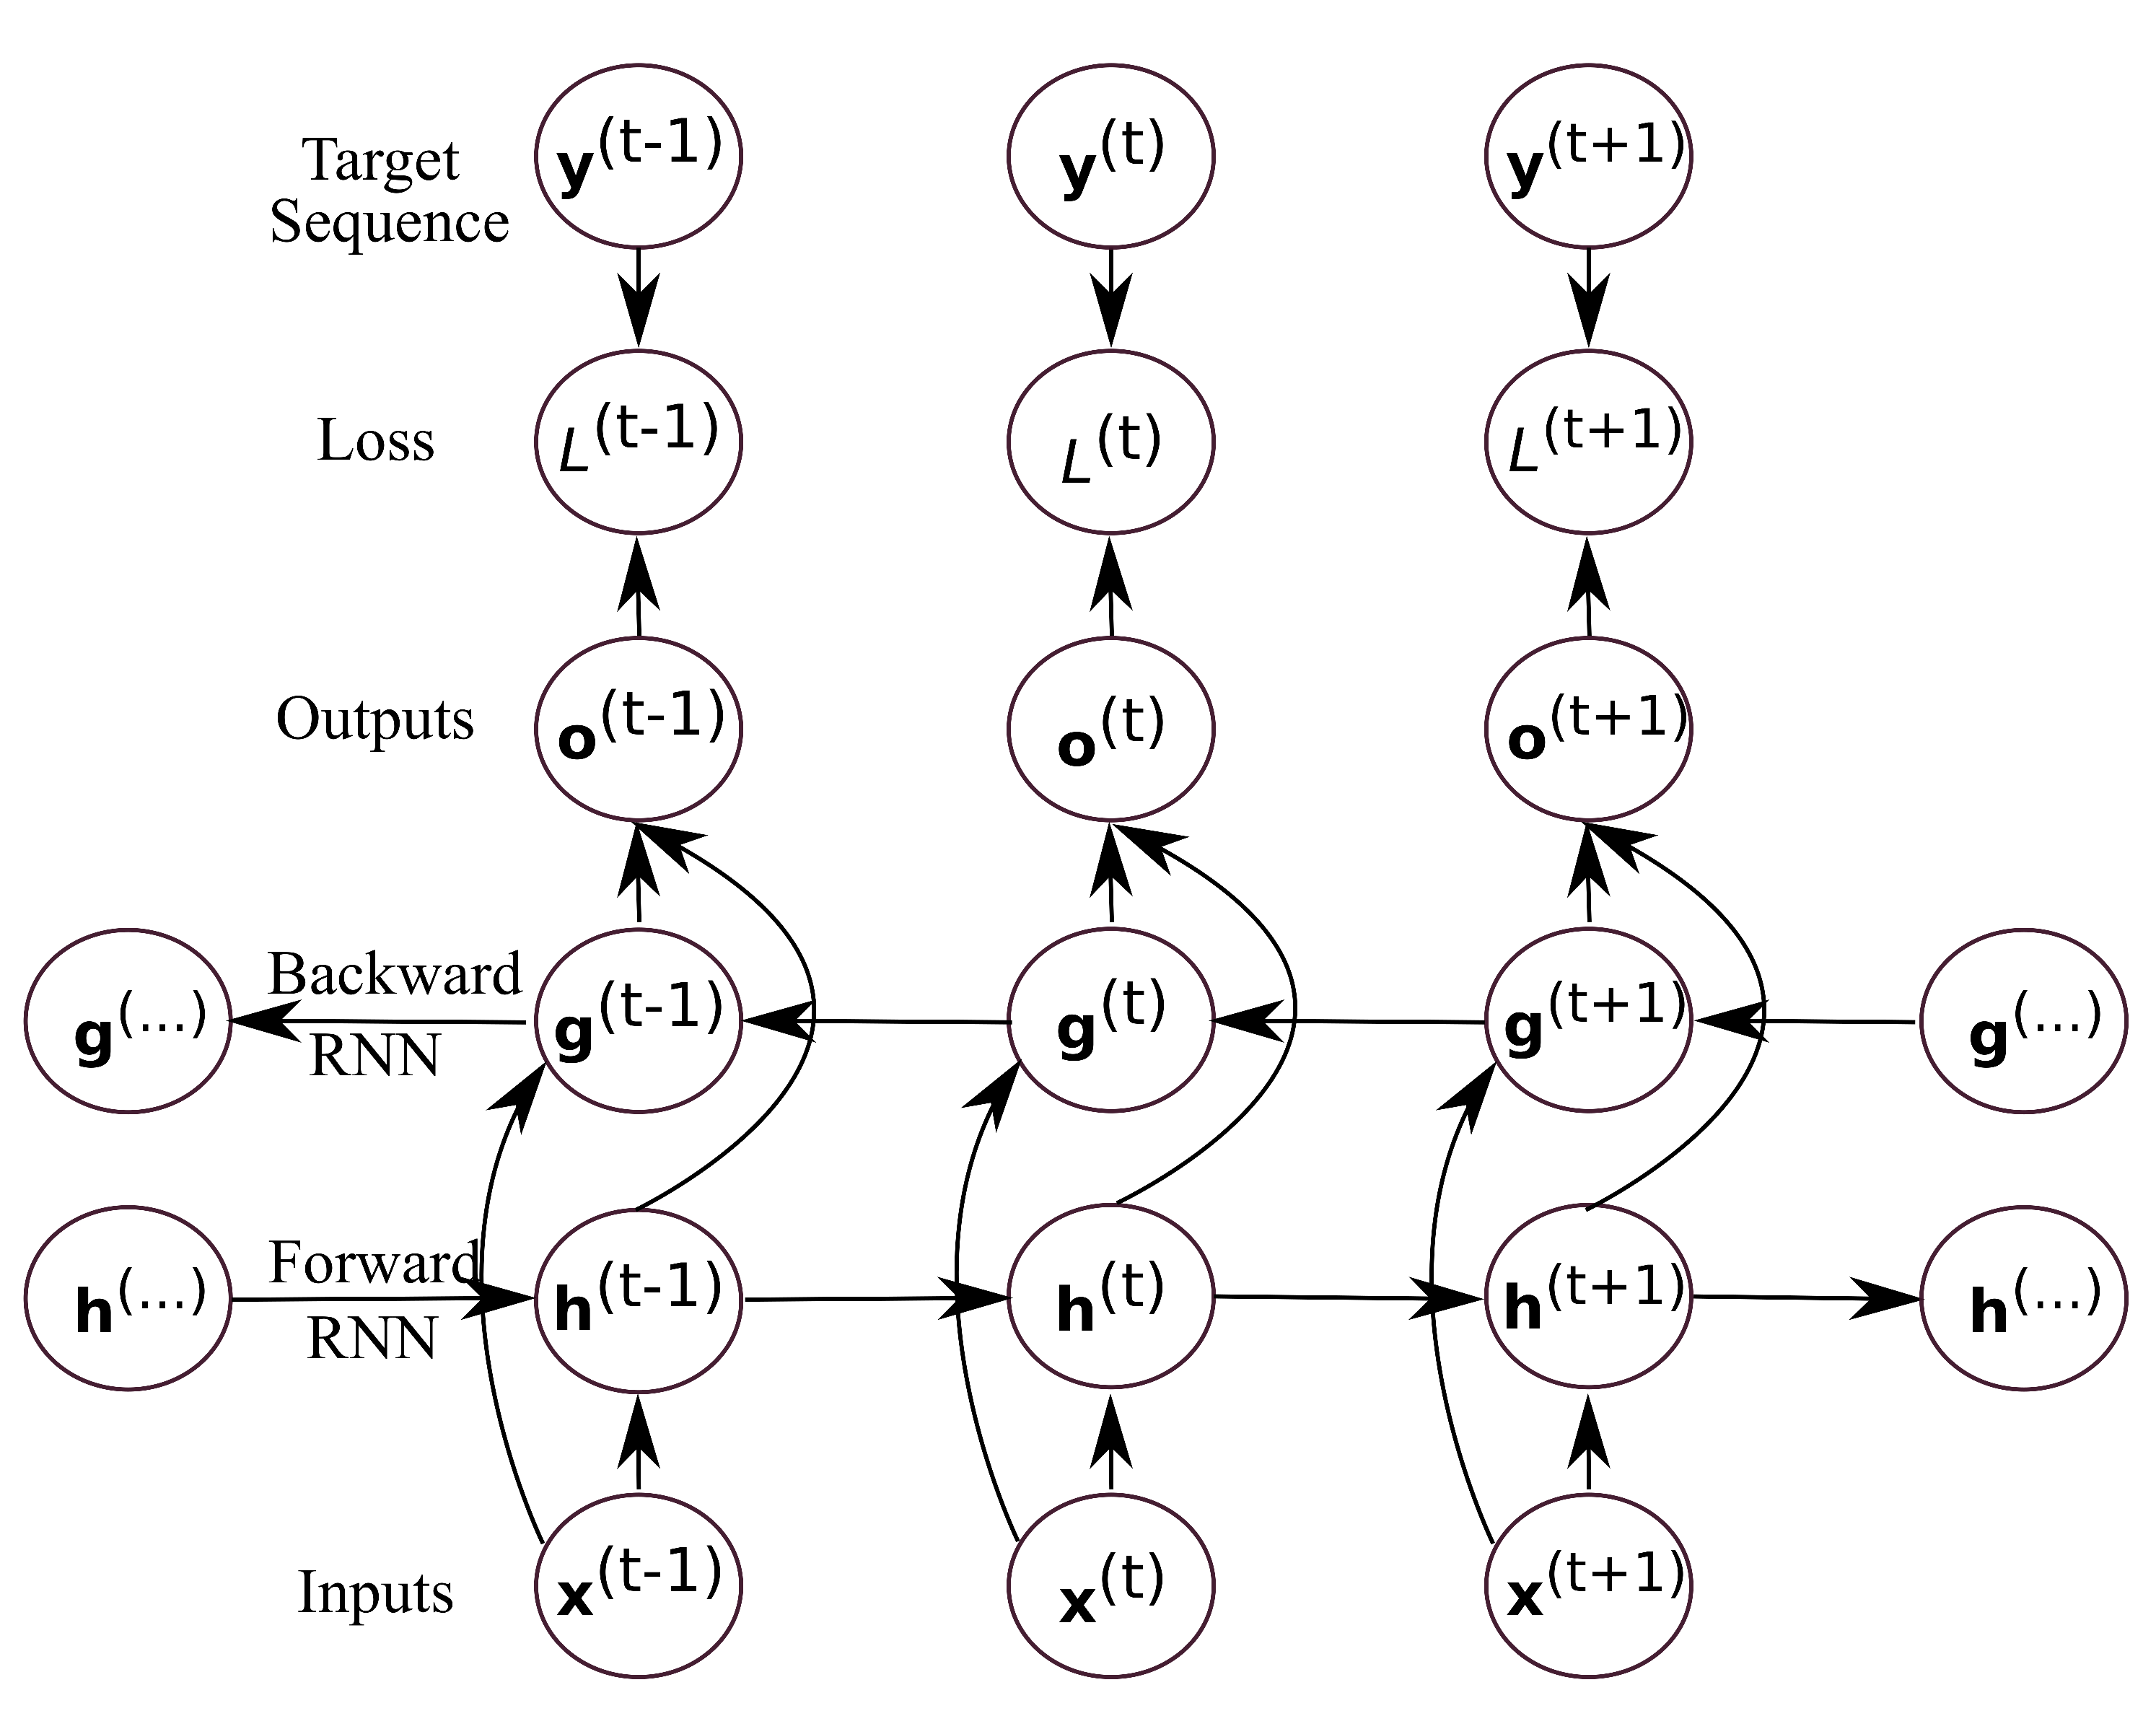
\includegraphics[width=0.9\textwidth]{figures/brnn.eps}
	\caption{Bidirectional RNNs \label{fig:bidirectional_rnn}}
\end{figure}
\subsubsection{Bidirectional GRU}

\subsection{Human Pose Estimation}
\subsubsection{Introduction to OpenPose Library} 
\subsubsection{Architecture and Details}



%-------------------------------------------------------------------------
\section{Extracting Spatio-Temporal Feature Vector}
Many strategies have been taken to designed a lower dimensional spatio-temporal feature descriptor based on the 2D human poses estimated from the raw video frames using an improved OpenPose~\cite{Cao_19} algorithm. In this section, we elaborate the feature extraction procedure of our proposed method. 


\subsection{2D Body Joints Feature}
As every joint of the human body does not have a significant role in gait pattern, they cannot improve gait recognition accuracy. Some joints perform even worse. So, among the 25 body joints estimated from OpenPose algorithm we searched out for those joints which have a rich and discriminative gait representation capacity. Cunado \textit{et al.}~\cite{Cunado_97} used the human leg-based model as they found that change of human leg contains the most important features for gait recognition.  In our study, we found that knee along with the joints located in the feet show more robustness than any other body joints because they do not alter while people are walking in cloths or carrying bags. For example, hip joints get wider in coat than normal condition. Again, in some gait videos, some subjects put their hands into their coat pocket, which they cannot do in normal walking. This situation significantly changes the joint coordinates. Furthermore, joints above hip joint do not have any significant impact on gait pattern. Hence, we do not consider hip or any other body joints above it.

\begin{figure}
	
	\centering 
	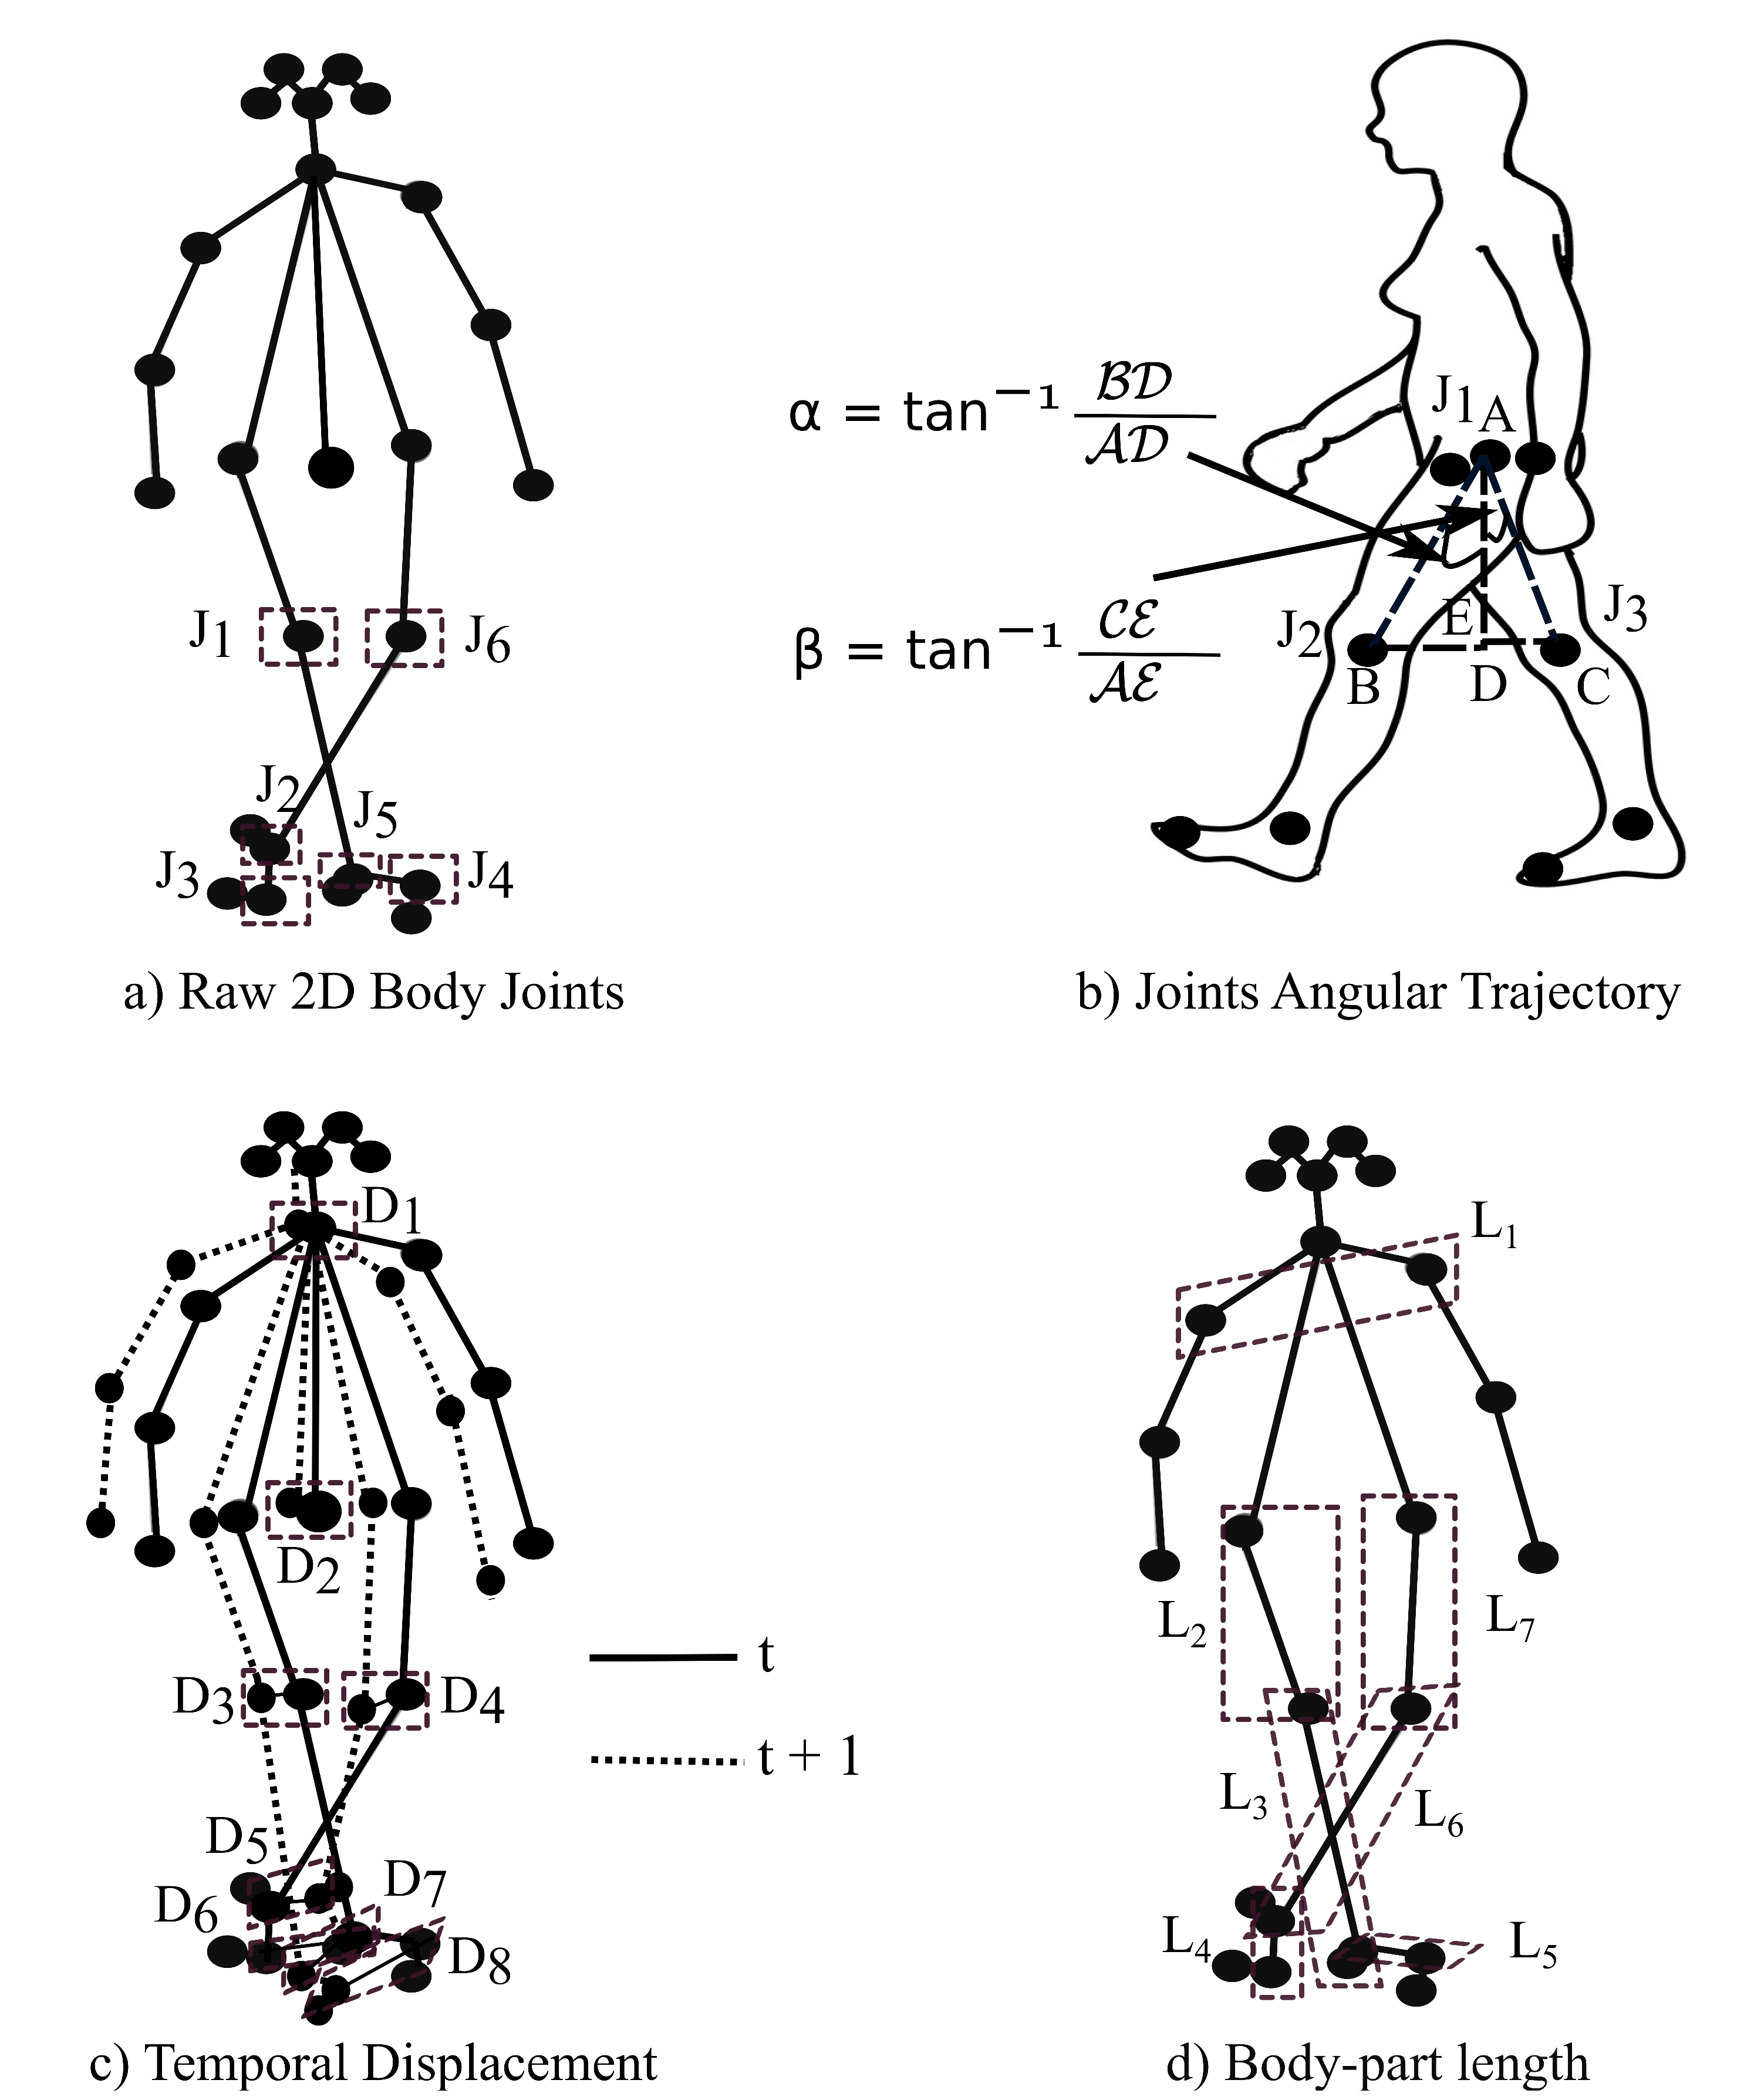
\includegraphics[width = 0.9\textwidth]{figures/extracted_features.eps}
	\caption[Different feature extraction process of the proposed method]
	{Different feature extraction process of the proposed method. a) 6 effective joints were selected out of 25 body joints as estimated from pose estimation algorithm~\cite{Cao_19}. These selected joints formed a 12-dimensional pose vector. b) 5 angular trajectories from lower limbs were considered to form a joint-angle feature vector. c) A total of 8 body joints were selected to get temporal displacement feature vector. d) 7 body parts were taken to form a limb length feature vector.\label{fig:extracted_features}
	}
\end{figure}

Consequently, in our work, as shown in Figure~\ref{fig:extracted_features}(a) we selected 6 body joints (RKnee, Rankle, RBigToe, LKnee, LAnkle, LBigToe) to form our effective pose features. Thus, we have 12-dimensional pose feature vector, $\textbf{f}_{pose}$, for a single frame. 

\begin{equation}
  \textbf {f}_{pose}= [x_1, y_1, x_2, y_2, \ldots\ldots, x_6, y_6]^T
\end{equation}

It is necessary to normalize the pose sequence data with regard to the subject position in frame, size, or speed of walking to get improved performance. In different gait datasets, as people walk through the fixed camera, the size of the subject's body alters due to change in the distance between the subject and the camera changes. In our study, to find the origin of the coordinate system ($J_c$) for each subject, we considered right, left, and middle of the hip joints and calculated the average of them. Again, to normalize the bodies of different subjects to a fixed size, we took $ h $, the euclidean distance from hip to neck joint, as unit length. Equation~\ref{equ:normalization_raw_join} shows the normalization procedure of the raw 2D joints.

\begin{equation} \label{equ:normalization_raw_joint}
\begin{split}
	Jc &= {(J_{LHip} +J_{RHip} +J_{MHip})} / {3} \\
	h &= \parallel {J_c} - {J_{neck}}\parallel_2  \\
	J_{i}^{N}  &= (J_i - J_c) / h 
\end{split}
\end{equation}
Here, ${J_i}^N$ be the new coordinate of the $i^{th}$ joint $J_{i}$ of a particular pose.


\subsection{Joint Angular Trajectory}
The dynamics of human gait motion can be expressed by the temporal information of joint angles. Hence, discriminative gait features can be found by considering the change in joint-angle trajectories of the lower limbs~\cite{Wang_04}. Therefore, in this study, we formulated a 15-dimensional feature vector $\boldsymbol{f}_{trajectory}$ by considering five lower limb joint-angle trajectories using following equations: 

\begin{table}
	\centering
	\caption{List of selected joint-angle trajectories with corresponding body joint set in order to form gait angular feature vector. \label{table:list_joint_angle_trajectory}}
	\begin{tabular}{cc}
		\hline
		\textbf{Angular Trajectory} & \textbf{Body Joints Set}\\
		
		\hline
		Hip trajectory &10, 8, 13 \\
		Right knee trajectory  &11, 10, 9 \\
		Left knee trajectory &14, 13, 12 \\
		Right ankle trajectory &22, 11, 10 \\
		Left ankle trajectory &19, 14, 13 \\
		\hline
	\end{tabular}
\end{table}

\begin{equation}
	\begin{split}
	\alpha &= 
	\begin{cases}
	\tan^{-1}{\frac{|J_{2,x}-J_{1,x}|}{|J_{2,y}-J_{1,y}|}} & J_{2,y} \neq J_{1,y}\\
	\pi/2 & J_{2,y} = J_{1,y}
	\end{cases} \\ \noalign{\vskip10pt}
	\beta &= 
	\begin{cases}
	\tan^{-1}{\frac{|J_{3,x}-J_{1,x}|}{|J_{3,y}-J_{1,y}|}} & J_{3,y} \neq J_{1,y}\\
	\pi/2 & J_{3,y} = J_{1,y}
	\end{cases} \\ \noalign{\vskip10pt}
	\theta &= \alpha + \beta
	\end{split}
\end{equation}

As shown in Figure~\ref{fig:extracted_features} (b), $J_1, J_2, J_3$ are the joints which form a set of angular trajectory. In this work, we considered five sets of angular trajectories from the lower limb of human body. Table~\ref{table:list_joint_angle_trajectory} demonstrated the selected angular trajectories with their corresponding body joints. For each trajectory, we took $(\theta, \alpha, \beta)$ as gait features. 

\begin{equation}
\textbf {f}_{trajectory}= [\theta_1, \alpha_1, \beta_1,\theta_2, \alpha_2, \beta_2,\ldots\ldots, \theta_5, \alpha_5, \beta_5]^T
\end{equation}


\subsection{Temporal Displacement}
Our third type of extracted features was a simple descriptor that preserves temporal information. It stores the local motion features of gait by keeping the displacement information between the two adjacent frames of the pose sequence. The displacement of each coordinate of a joint was then normalized by the total length of displacement of all joints. Let, $ t $ and $ (t + 1) $ are two adjacent frame of a particular gait. The displacement information of the coordinates of any joint of frame $ t $ would be the normalized difference between the corresponding coordinates. 

\begin{equation}
\begin{split}
\triangle x^{t}_{1} &=\frac{x^{t+1}_{1} - x^{t}_{1}}{\sum_{i=1}^{8}\parallel J^{t+1}_{i} - J^{t}_{i}\parallel_2} \\ 
\triangle y^{t}_{1} &=\frac{y^{t+1}_{1} - y^{t}_{1}}{\sum_{i=1}^{8}\parallel J^{t+1}_{i} - J^{t}_{i}\parallel_2} \\ 
{\bf f}_{displacement} &= [\triangle x_{1}, \triangle y_{1}, \triangle x_{2}, \triangle y_{2} \ldots\ldots, \triangle x_{8}, \triangle y_{8}]^{T}
\end{split}
\end{equation}

Here, $J_i^{t}$ is the 2D coordinates of the $i_{th}$ body joint at $t^{th}$ frame in the video and $(\triangle x_1^t , \triangle y_1^t )$ is the displacement of the coordinates of first joint at $t^{th}$ frame of the video. As shown in Figure~\ref{fig:extracted_features} (c), we selected 8 joints (Neck, MHip, RKnee, Rankle, RBigToe, LKnee, LAnkle, LBigToe) to get a 16-dimensional feature vector, $\textbf{f}_{displacement}$.


\subsection{Body Part Length Features}
The static gait parameters, for example, the length of the body parts calculated from raw body joints position are also important for gait recognition~\cite{Wang_04, Araujo_13}. They form a spatial gait features which make them robust against covariate such as carrying and clothing variation. In this study, we took seven body parts (Figure~\ref{fig:extracted_features} (d)) namely length of the two leg, two feet, two thigh and width of the shoulder which formed a 7-dimensional spatial feature vector $\textbf{f}_{body-part}$. 


\subsection{Fusion of Features}
A Lot of research works have been done to fuse multiple features to get improved performance~\cite{Liao_19, Wang_04}.  Different types of fusion methods were proposed in literature such as feature level fusion, representation level fusion, and score level fusion. In feature level fusion, multiple features of the same frame are concatenated before feeding into a final network and in representation level fusion, each feature vector is firstly fed into a network and the resulting global representations are then concatenated to train a final classifier. For score level fusion, each feature vector is separately fed into the final network which predicts a classification score. Then, the scores from multiple classifiers are fused using an arithmetic mean.

In this study, we found that feature level fusion has produced better recognition results in contrast to other fusion techniques or individual feature sets. 


\begin{figure}
	\centering 
	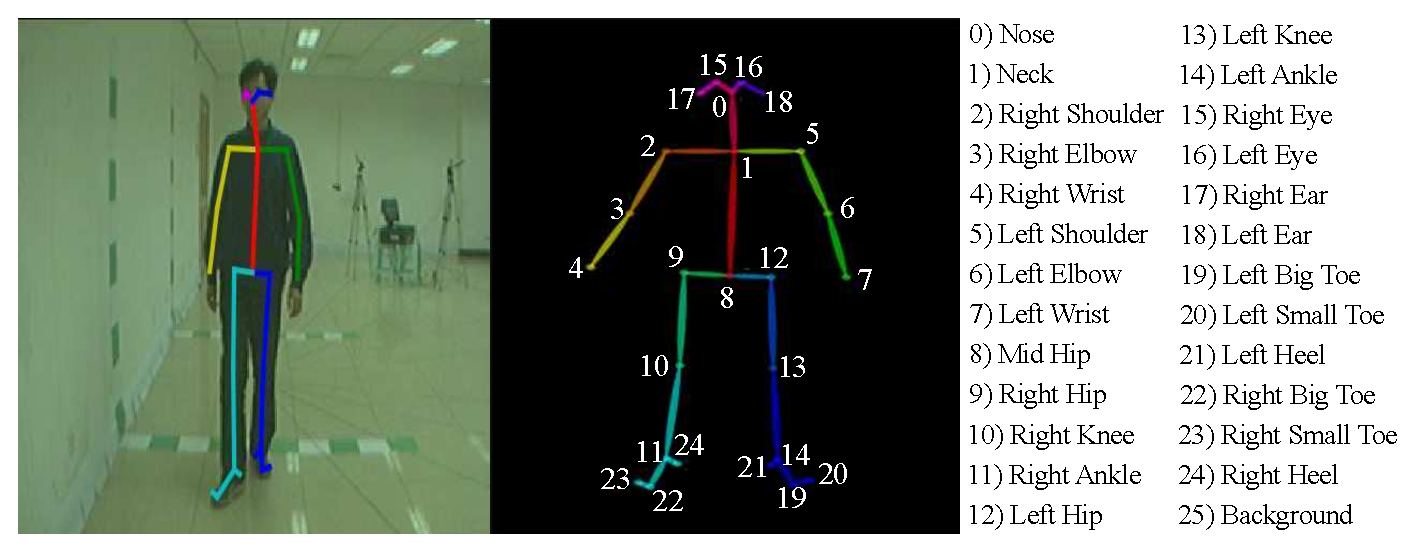
\includegraphics[width = 0.9\textwidth]{figures/pose_estimation.eps}
	\caption[Examples of 2D human pose estimation from RGB images of CASIA dataset]
	{Examples of 2D human pose estimation by~\cite{Cao_19} from RGB images of CASIA dataset (left ones). Detected 25 human body joints with description are shown. (right ones) \label{fig:pose_estimation}
	}
\end{figure}

%-------------------------------------------------------------------------
\section{Feature Preprocessing}
From 2D pose estimation algorithm~\cite{Cao_19}, we got 25 body joints from each frame (Figure~\ref{fig:pose_estimation}). 

\subsection{Handling Missing Data}
We took several preprocessing steps to address the problem of missing data due to occlusions. The main strategies are: 
\begin{itemize}
\item If the origin of the coordinate system can't be calculated due to missing hip joints, the frame should be rejected.
\item If more than 1 body joint is missing in between knee and ankle joints of both leg, the frame should be rejected due to having little information.
\item In other cases, individual joints were not located in the frame and a position of $[0.0, 0.0]$  was given to that joint. 
\end{itemize}

The above strategies are simpler which do not require any computation and proven to be effective in addressing the missing data problem.

\subsection{Forming Feature Map}
In this research, we designed a 50-dimensional spatio-temporal gait feature vector \textbf{p} from the raw 2D pose estimation of each frame.  Firstly, we split a gait video into 28 frame segments. Each 28 frame-segment formed a timestep which can be described by equations~\ref{equ:feature_preprocess}. Here, \textbf{p} is 50-dimension pose vector for each frame; \textit{\textbf{T}} is the feature matrix for each timestep; $ N $ is the total number of timestep sequence, and \textit{\textbf{V}} is the sequence of features for a gait video. 

\begin{equation}
\label{equ:feature_preprocess}
\begin{split}
\boldsymbol{p} &= {[f_1, f_2, f_3, \ldots \ldots, f_{50}]}^T \\
\boldsymbol {T} &= {[\boldsymbol p_1, \boldsymbol p_2, \boldsymbol p_3,  \ldots \ldots, \boldsymbol p_{28}]}^T \epsilon \quad \mathbb {R}^{28\times 50}\\
\boldsymbol V &= {[\boldsymbol T_1, \boldsymbol T_2, \boldsymbol T_3,  \ldots \ldots \boldsymbol T_{N}]}^T 
\end{split}
\end{equation}


\subsection{Data Augmentation}
The performance of deep neural networks is strongly correlated with the amount of available training data.  Although CASIA~\cite{Yu_06} is the largest gait dataset, the standard experimental setup of this dataset(see Table ~\ref{table:caisab_setup}) allows us to train only the four normal walking sequence for each subject. Therefore, we need to augment our train data to obtain a stable model.  
One way to increase the amount of training data is to overlap video clip. So, we split the input video into an overlapping sequences of video clips. For every 28 image clip, we overlapped 24 images of the previous clip at almost $ \textbf{85.7\%} $ overlapping rate. For example, a particular gait video of 100 frames would be split into the clips $(1-28), (5-32), (9-36), ...$ up to frames $(73, 100)$. 

Again, in CASIA dataset, gait videos of different subject have varying timesteps. The number of timesteps in each gait video depends on the total number of frames where a person is detected. Due to the position of the camera, some angles ${(0^{\circ}, 18^{\circ}, 36^{\circ})}$ have more person detected frame than other angles ${(72^{\circ}, 90^{\circ}, 108^{\circ})}$. Therefore, the total number of timesteps in a gait video is different for different subjects and view angles. This varying timestep makes our train dataset unbalanced. Again, in CASIA B dataset, not all subjects have all gait videos; there are some missing gait videos. To solve the problem, we develop our own balance training set by making each subject pose sequence to have a fixed number timesteps. We first found the subject which had maximum timesteps for a particular gait angle and then augmented other subject's timesteps with that specific length by overlapping their sequences.

In addition to above technique, we further augment our training data by adding another gait sequence (i.e., $ 25\% $ increment) by implementing Gaussian noise to a given normal walking sequence. 

\begin{equation}
N(j_i) = (x + \tilde{x},  \quad y+ \tilde{y})
\end{equation}

Here,  $\tilde{x}$ and $\tilde{y}$ are two random real numbers generated by a normal distribution with zero mean and unit standard deviation. We apply noising (N) into the raw joints position of a training pose data.


%-------------------------------------------------------------------------
\section{Single-View Gait Recognition}
In this section, we will present the details of the architecture and training procedure of our proposed network for single-view gait recognition. We will also try to describe why our proposed 2-layer BiGRU network is best in modeling the gait descriptors for recognizing the subject ID.

\subsection{Network Architecture}
\begin{figure}
	\centering 
	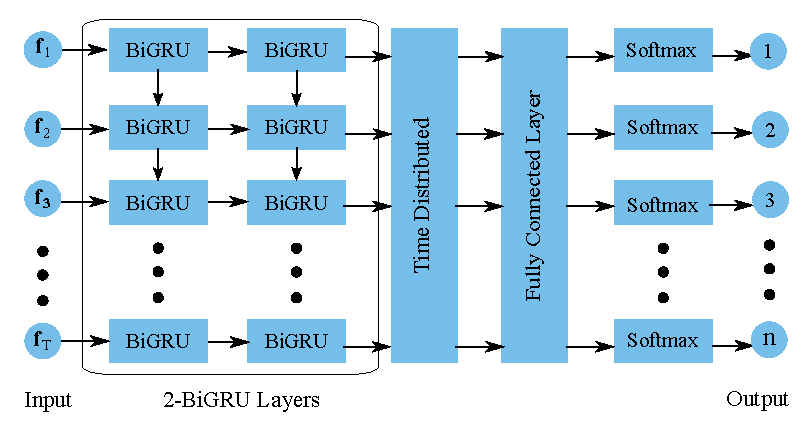
\includegraphics[width = 0.8\textwidth]{figures/rnn_network.eps}
	
	\caption[Proposed RNN architecture for robust gait recognition]
	{Proposed \gls{rnn} architecture for robust gait recognition. It consists of two \gls{bigru}~\cite{Schuster_97} layers each of which consists of $ 80 $ \gls{gru} cells with one batch normalization and one output softmax layer. The network was fed with a 50-dimensional spatio-temporal feature vector obtained from 2D pose estimation. Input layer was followed by a batch normalization layer~\cite{Ioffe_15}. The output of the recurrent layers was also batch normalized to standardize the activations and finally fed into an output softmax layer. For the output layer, the number of the output neuron equals to the number of subjects. \label{fig:rnn_network}
    }
\end{figure}


In this research, we experimented with different \gls{rnn} architectures such as Gated Recurrent Units (\gls{gru}s),  Long Short-Term Memory Units (\gls{lstm}s), Bidirectional Long Short-Term Memory (\gls{bilstm})~\cite{Graves_05} and Bidirectional Gated Recurrent Units (\gls{bigru})~\cite{Schuster_97}. Firstly, we designed the proposed network employing all these architectures with one recurrent layer and then, searched for optimum recurrent unit size between 50 to 150. Thereafter, we increased the capacity of the network by adding the second and third layers of hidden units. Finally, we found that, among different RNN architectures, 2-layer BiGRU with 80 hidden units performs best. 

After input and the second recurrent layer, we placed a batch normalization (\gls{bn})~\cite{Ioffe_15} layer. At last, a fully connected layer with softmax activation was used to predict the subject classes. Figure~\ref{fig:rnn_network} illustrates the architecture of the proposed network. 


\subsection{Training}
The training of \gls{rnn}s allows us to learn the parameters from the sequence. We have employed Adam~\cite{Kingma_15} optimization algorithm with $\beta_1 = 0.9, \beta_2 = 0.999$, which is known to work very well for training recurrent neural networks. We tried several learning rates in our experiment and found out that the best initial learning rate is $(1$x$10^{-3})$. We also reduced the learning rate by a factor when it hit a plateau. Reducing the learning rate will allow the optimizer to get rid of the plateaus in the loss surface. Table~\ref{table:summary_tn} summarizes all the hyperparameters setting of our network.

\begin{table}
	\centering
	\caption{Training summary of our proposed temporal network. \label{table:summary_tn}}
	\begin{tabular*}{32pc}{@{\extracolsep{\fill}}ll@{}}
			\hline \noalign{\vspace{3pt}}
			\textbf{Hyperparameter} &\qquad \textbf{Value} \\ [3pt] \hline\noalign{\vspace{3pt}}
			Optimizer     			&\qquad Adam~\cite{Kingma_15} \\[3pt]
			Objective function  	&\qquad Fusion of softmax and center loss \\[3pt]
			Epochs        			&\qquad $ 450 $ \\ [3pt]
			Initial learning rate	&\qquad $5 \times 10^{-3}$  \\[3pt]
			Mini-batch size			&\qquad $ 256 $ \\
			\hline
	\end{tabular*}
\end{table}

The proposed network was trained with a batch size of $ 256 $ for $ 450 $ epochs. Our network showed some overfitting mostly due to the high learning capacity of the network over data. This overfitting problem has been addressed by adding a batch normalization layer. We also tried to add dropout layer during training, but that did not help to reduce the overfitting problem. Moreover, it degraded gait recognition performance. Hence, we skip it.


\subsection{Loss Functions}
In this work, we found that due to the influence of various covariate factors, intraclass distance related to one subject is sometime more significant than interclass distance. Now, if we only use the \textit{cross-entropy loss} (\gls{ce}) as our objective function, the resulting learned features may contain large intraclass variations. Therefore, to effectively reduce the intraclass distance, we used \textit{center loss} (\gls{cl}), introduced by Wen \textit{et al.}~\cite{Wen_16} for face recognition task. As the training progresses, the center loss learns a center for features of each class and the distances between the features and their corresponding class centers are minimized simultaneously. However, using only center loss may lead the learned features and centers close to zeros due to the very small value of the center loss. Hence, with the fusion of softmax loss ($L_s$) and center loss ($L_c$), we can achieve discriminative feature learning by increasing interclass dispersion and compacting intraclass distance as much as possible.


\begin{equation} \label{equ:loss_functions}
\begin{split}
L_s &=-\sum_{i=1}^{m}log{\frac{e^{W_{y_i}^{T}x_i + b_{y_i}}}{\sum_{j=1}^{n}{e^{W_{j}^{T}x_i+ b_j}}}} \\
L_c &= \frac{1}{2}\sum_{i=1}^{m}{\parallel{{\boldsymbol x_i}-{\boldsymbol c_{y_i}}}\parallel}_2^2 \\
L &= L_s + \lambda L_c + \lambda_{\theta}\parallel{\theta}\parallel_{2}
\end{split} 
\end{equation}

Equations~(\ref{equ:loss_functions}) describe the total loss ($ L $) calculation of our network. where $\boldsymbol x_{i} \epsilon \mathbb {R}^d$ denotes the $i^{th}$ pose sequence which belongs to the $y_i^{th}$ class and  $\boldsymbol c_{y_i} \epsilon \mathbb {R}^d$ denotes to the $y_i$th class center of the learned pose features. $W \epsilon \mathbb {R}^{d\times n}$ is the feature dimension of the last fully connected layer and $b\epsilon \mathbb {R}$ is the bias term of the network. The batch size and the class number are $ m $ and $ n $ respectively. $\lambda$, a scalar variable, is set to value $ 0.01 $ to balance the two loss functions. $\parallel{\theta}\parallel_{2}$ refers to the kernel regularizer for all the parameters of the network with a weight decay coefficient $(\lambda_{\theta})$ set to $0.0005$ for the experiment.  


\subsection{Post-processing}\label{subsec_post_process}
While training, our proposed temporal network considers each of these video clip as a separate video (see Fig.~\ref{fig:output_prediction}). For a given video, the prediction of our model is a sequence of class probabilities for each of the timestep, i.e. 28 frame clip.

\begin{figure}
	\centering
	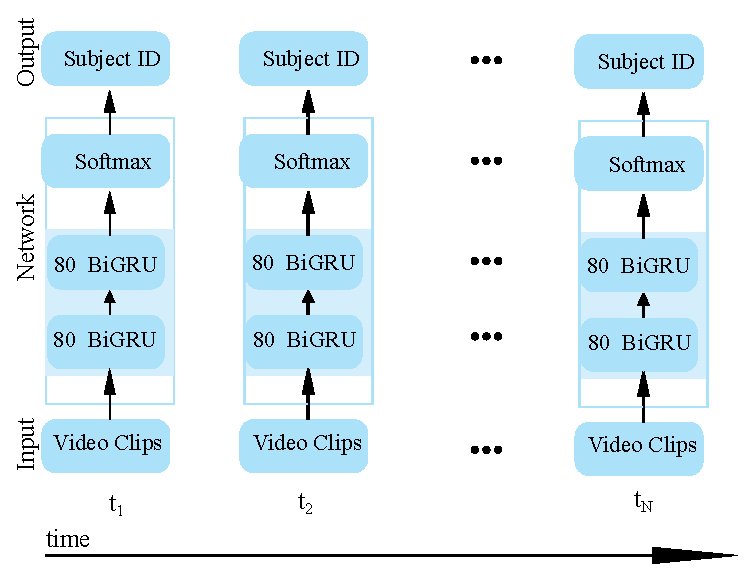
\includegraphics[width=0.7\textwidth ]{figures/output_prediction.eps}
	\caption[Output prediction scheme of our proposed temporal network]{
		Output prediction scheme of our proposed temporal network. Each input clip was considered as a separate video and a sequence of class probabilities was predicted at output. \textit{Majority voting scheme }was used to process the output to predict the subject ID.
	}
	\label{fig:output_prediction}
\end{figure}

But, while testing, we actually need the subject ID for the complete gait video. Therefore, we used \textit {Majority voting scheme} to process this output to predict the subject ID. In this scheme, the subject that receives the highest number of votes over all timesteps in a  gait video is referred as the predicted class.

Let\rq s consider, $\boldsymbol{s}$ is a vector of $n$ number of subjects. For a particular timestep $t$ of a gait video, input pose sequence vector $\boldsymbol X^t \epsilon \mathbb {R}^{28\times 50}$ has an n-dimensional output vector $\boldsymbol o^t$.

\begin{equation} \label{equ:timestep_sequence}
\begin{split}
\boldsymbol s^t &=  {[s_1, s_2, s_3, ....., s_{n}]}^{T}\\
\boldsymbol o^t &=  {[o_1, o_2, o_3, ....., o_{n}]}^{T}
\end{split}
\end{equation}

Here, $o_i^t = P(s_i | X^t)$ refers the probability of input feature map $\boldsymbol X^t$ belongs to class $s_i$. Now, we assign the output class $s^t$ to the subject class $s_i$ which have maximum probabilities for the timestep $t$. As each of our gait videos is divided into a series of timestep sequence (see equation~\ref{equ:timestep_sequence}), using majority voting scheme we can have the subject ID. Following equations described the voting scheme:

\begin{equation}
\label{equ:predicted_class}
\begin{split}
s_t &=  \arg\max_{s_i}{\{o_i^t | 1 \leq i \leq n\}} \\
s &= {\arg\max}_{i\in(1, 2, ...,n)}{\sum_{t=1}^{N}s_i^N}
\end{split}
\end{equation}

Here, $ N $ is the total number of timesteps in which a gait is split and $ s $ is the final predicted class.  



%-------------------------------------------------------------------------
\section{Multi-View Gait Recognition}
The workflow of our proposed two-stage multi-view gait recognition network is illustrated in Fig.~\ref{fig:multi_view_gait_recognition}. In first stage, we trained a 3D convolutional network to estimate the walking direction of the subject by extracting spatio-temporal features from gait video. Thereafter, we performed subject recognition using proposed temporal network which has been trained for that particular angle.


\subsection{Preprocessing}
Firstly, to localize human walking in gait videos, we used YOLOv3, a state-of-the-art real-time object detection algorithm, proposed by Redmon \textit{et al.}~\cite{Redmon_18}. We then cropped each of the person detected frame using the bounding box coordinates found from YOLOv3 algorithm and resized them to $112\times112$ for our network input. Thereafter, we splitted each gait video into overlapping sequences of 16 consecutive frames within training or test set. There is an overlap of 8 frames (50\%) indicating that the samples were gathered using a 16 frame sliding window with a 50\% stride.


\begin{figure}
	\centering
	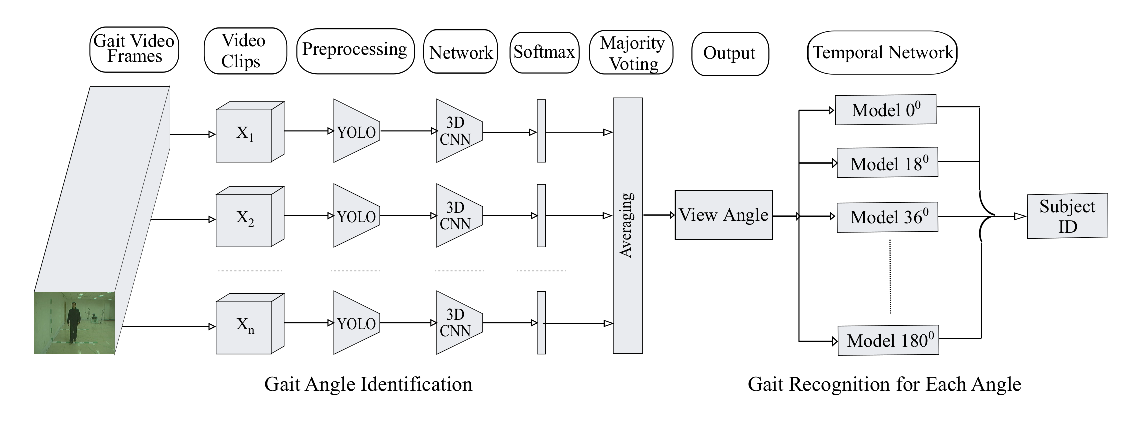
\includegraphics[width=\textwidth]{figures/multi_view_gait_recognition.eps}
	\caption[Overview of our proposed multi-view gait recognition network scheme] 
	{Overview of our proposed multi-view gait recognition network scheme. YOLOv3~\cite{Redmon_18} was used to detect and locate the walking people in video frames. The input of the network was a clip of 16 consecutive frame which was preprocessed and resized to $112\times112$ to feed into a 3D convolutional network based on C3D~\cite{Tran_15}. The network used 3D kernels to exploit spatio-temporal dynamics for viewing angle identification. Thereafter, a temporal network, trained on each viewing angle, was performed subject identification by modeling temporal dynamics from input 2D pose sequence. \label{fig:multi_view_gait_recognition}
	}
	
\end{figure}

\subsection{Network Architecture}
Identifying walking direction from gait video is somewhat similar to action recognition problem in computer vision. Recently, in action recognition, researcher have started to exploit 3D features in video using 3D-CNN model which extracts features from both spatial and temporal dimensions by performing 3D convolutions. Tran et.al.~\cite{Tran_15} proposed a 3D convolutional neural network, also known as C3D, which has been widely used for applications like video classification, action recognition, etc. This network has been trained on one of the largest video classification benchmark datasets Sports-1M~\cite{Karpathy_14}. The dataset contains 1.1 million sports videos, where each video belongs to one of the 487 sports categories. 

The proposed method for our gait angle identification is illustrated in Fig.~\ref{fig:multi_view_gait_recognition}. The input of the network was a clip of 16 consecutive frame which was preprocessed and resized to $112\times112$ to feed into a a 3D-CNN network. We used {\textit {majority voting scheme}} to process the output to predict the view angle similar to section~\ref{subsec_post_process}, i.e. the angle that receives the highest number of votes over all clips are referred as predicted angle of the video.

\begin{figure}
	\centering {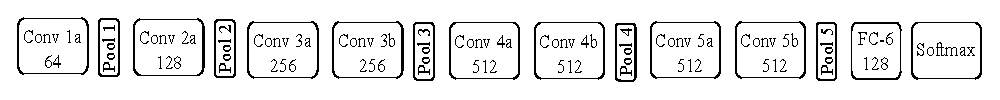
\includegraphics[width=\textwidth]{figures/3D_CNN.eps}}
	\caption[Proposed 3D-CNN for video angle identification]
	{Proposed 3D-CNN for video angle identification. Last 3 layers of a pretrained C3D~\cite{Tran_15} network has been replaced by a fully connected layer of 128 neurons followed a final softmax layer of 11 neurons to classify 11 different walking direction in CASIA-B dataset. \label{fig:3D_CNN}
	}
	
\end{figure}

\begin{table}
	\centering
	\caption{Training summary of our proposed 3D-CNN network.  \label{table:summary_3dcnn}}
	\begin{tabular*}{30pc}{@{\extracolsep{\fill}}ll@{}}
			\hline \noalign{\vspace{3pt}}
			\textbf{Hyperparameter} & \textbf{Value} \\ \hline\noalign{\vspace{3pt}}
			Optimizer  &Stochastic gradient descent (\gls{sgd})  \\ [3pt]
			Objective function  &Mean squared error (\gls{mse}) \\ [3pt]
			Epochs  &70  \\ [3pt]
			Initial learning rate & $1 \times 10^{-3}$ \\ [3pt]
			Mini-batch size	  &12  \\ [3pt]
			Momentum  &0.92 \\ [3pt]
			\hline
	\end{tabular*}
\end{table}

Successful transfer learning within or across different domain of interest leads to significant improvement in performance due to the amount of jointly learning representations in a shared feature space. In our work, we used a pretrained C3D model and fine-tuned it for our 3D Convolutional network to determine the viewpoint angle from gait videos. Fig.~\ref{fig:3D_CNN} shows our proposed 3D convolutional network. 

C3D network is composed of 8 convolutional layers, 5 pooling layers, 2 fully-connected layers, followed by a softmax layer at the end. All the 3D convolution kernels are $3\times3\times3$ with stride 1 in both spatial and temporal dimensions. We removed the last 3 layer from the model and then added a fully connected layer of 128 neurons and a dropout layer of 0.5 to avoid overfitting. Finally, a softmax layer of 11 neuron has been added to classify any given videos into 11 different viewing angles. 


\subsection{Training}
We used CASIA-B gait dataset~\cite{Yu_06} to train our model. We trained the network using 4 normal walking sequences of 100 subject in gallery set of CASIA-B as described in Table~\ref{table:caisab_setup}. Our network was trained with a 12 batch size with an initial learning rate ${10^{-3}}$ for 70 epochs. Table~\ref{table:summary_3dcnn} summarizes all hyper-parameters setting of our proposed network.


